%!TEX root = ../dokumentation.tex
\chapter{Reaktion auf Hindernisse}
Reaktion kommt vom alt-lateinischen \textit{reactio} und bedeutet Rückhandlung. Genauer bedeutet es sein eigenes Verhalten an Etwas anzupassen. Lebewesen reagieren auf Umwelteinflüsse auf der Basis von Annahmen und Erfahrung. Diese Erfahrung wird durch wiederholtes Analysieren unterschiedlichster Situationen gewonnen. Die Annahmen bestehen aus dem Vergleich und der Kombination von Erfahrungen. Ein Roboter selbst, ist dazu allerdings nicht in der Lage. Ein solches Verhalten kann allerdings an trainiert werden. Dazu müssen die Merkmale zum deuten der Situation und die adäquate Verhaltensweise vorgegeben werden. Diese Informationen können durch das Modellieren einer solchen Situation erhoben werden.

%\begin{itemize}
%\item was bedeutet reagieren?
%\item Situation analysieren; Annahmen treffen
%\item eigenes Verhalten anpassen anhand getroffener Annahmen
%\item Annahmen beruhen auf Erfahrung
%\item Erfahrung durch stetige Beobachtung von Situationen und Analyse der Ergebnisse
%\item Roboter selbst kann so etwas nicht
%\item Verhalten kann aber an trainiert werden
%\item dazu müssen Verhaltensweise und Merkmale zum deuten der Situation gegeben werden
%\item Eventueller Lösungsweg durch Systemmodellierung via Bayes'sches Netz
%\end{itemize}
\section{Modellierung von Situationen}
Eine Situation kann als geschlossenes System betrachtet werden. An einer Situation sind unterschiedliche Elemente beteiligt. Jedes Element verhält sich unterschiedlich. Jedes Element weist zudem verschiedene Verhaltensmuster auf. Ein System enthält Variablen. Jede Variable kann verschiedene Zustände annehmen. Somit lässt sich eine Abbildung von Elementen auf Variablen durchführen. Die Verhaltensmuster eines Elements sind die Zustände einer Variable. Ein Beispiel hierfür lässt sich anhand des Roboters und seines Verhaltens aufzeigen. Der Roboter selbst ist eine Variable. Der Roboter soll sich innerhalb eines Raumes auf dem Boden bewegen. Sein Zustand ist während dem er sich bewegt \textit{moving}. Er bewegt sich jedoch nicht die ganze Zeit, sondern nur wenn er einen Auftrag bekommt, sich an eine Position zu begeben. Wenn er sich nicht bewegt wartet er auf einen Auftrag. Somit ist ein weiterer Zustand \textit{waiting}.
%\begin{itemize}
%\item Was ist eine Situation; Kann als geschlossenes System betrachtet werden;
%\item Situation enthält teilnehmende Elemente; Elemente weisen ein Verhalten auf;
%\item Elemente bilden die Variablen eines Systems dar; Das Verhalten wiederum der Zustand dieser Variable; Für jedes Verhaltensmuster ein eigener Zustand
%\end{itemize}

%\begin{itemize}
%\item Roboter = Variable
%\item Roboter bewegt sich im Raum; Zustand = moving;
%\item Roboter steht still; Zustand = fixed;
%\end{itemize}
Die Abbildung von Hindernissen innerhalb des Systems ist allerdings nicht ohne weiteres möglich. Dies liegt daran dass sich Störobjekte nicht die ganze Zeit im Raum befinden. Sie betreten den Raum, bewegen sich darin und verlassen Ihn eventuell wieder. Dieser Fall kann nicht als System dargestellt werden, da dessen Variablen ein fester Teil davon sind. Ein Lösungsansatz für dieses Problem wäre eine Unterteilung in verschiedene Situationen und damit auch in verschiedene Systeme. Der Wechsel zwischen den Teilsystemen kann Anhand anschließend durch Fallunterscheidungen erfolgen. Als Basis für die Fallunterscheidung wird nun eine Klassifikation der Hindernisse vorgenommen und darin deren erwartetes Verhalten definiert.
%\begin{itemize}
%\item Schwieriger bei Störobjekten
%\item Objekte sind nicht die ganze Zeit da
%\item Wenn sie da sind unterschiedliches Verhalten
%\item Variablen in einem geschlossenen System verschwinden nicht und tauchen nicht einfach auf
%\item Allerdings spricht nichts gegen die Abbildung auf mehrere Systeme und dem Wechsel zwische Ihnen basierend auf Fallunterscheidungen.
%\end{itemize}

\section{Klassifikation}
Eine Klassifikation beschreibt zunächst das zu modellierende Setting und dessen erwartete Ereignisse. Anschließend werden auf Basis der beschriebenen Szenarios Muster abgeleitet. Ebenfalls offenbaren sich Merkmale wie messbare Einheiten, welche für Systemwechsel herangezogen werden können.\\
In diesem Fall werden die Ereignisse welche durch das Auftauchen von Hindernissen getriggert werden beleuchtet. Ein Fall kann zu diesem Zeitpunkt bereits abgeleitet werden. Dadurch dass Hindernisse auftauchen muss es ein System geben in dem kein Hindernis im Raum existiert. Dieser Fall kann als initiales System angesehen werden. Objekte welche den Bewegungsraum des Roboters betreten sind zu diesem Zeitpunkt in Bewegung. Sie können sich auf unterschiedliche Art bewegen. Zum einen auf einem geraden Pfad. Zum anderen verfolgen sie keinen ersichtlichen Pfad, stattdessen bewegen sie sich willkürlich durch den Raum. Statt den Raum zu verlassen kann ein Objekt auch die Bewegung unterbrechen und eine fixe Position innerhalb des Raumes annehmen. Zuletzt besteht die Möglichkeit dass ein Objekt die Grenzen des Raums nur streift, und ihn nur für einen kurzen Zeitpunkt betritt und sofort wieder verlässt.\\
Anhand des Settings können nun folgende Klassen von Hindernissen geschaffen werden.

%\begin{itemize}
%\item Klassifikation enthält zunächst die Erwarteten Ereignisse
%\item Welche Muster lassen sich daraus ableiten?
%\item welche Messwerte Messwerte/Merkmale können innerhalb der Situation beobachtet werden?
%\item Wie können die erwarteten Messwerte/Merkmale genutzt werden um eine Fallunterscheidung durchzuführen?
%\item Anhand des Settings wurden nun folgende Kategorien für Hindernisse geschaffen
%\end{itemize}
\begin{itemize}
\item \textbf{lineare Objekte} bewegen sich auf einem festen geraden Pfad durch den Raum.
\item \textbf{dynamische Objekte} bewegen sich auf keinem ersichtlichen Pfad durch den Raum.
\item \textbf{statische Objekte} sind entweder lineare oder dynamische Objekte welche die Bewegung abgebrochen haben und an einer festen Position innerhalb des Raumes verweilen.
\item \textbf{periphere Objekte} streifen den Bewegungsraum des Roboters nur oberflächlich, und verlassen ihn sofort wieder.
\end{itemize}

\subsection{Konzept Bewegungsanalyse}
Die Klassifizierung der aufgeführten Objekte basiert auf deren Bewegungsmuster. Eine Voraussetzung für die Implementierung dieser Klassen besteht darin die Bewegung von Objekten nachvollziehen zu können. Die Bewegung selbst stellt sich als Positionsänderung zwischen zwei Frames dar. Das Problem liegt hier nun darin eine Verbindung zwischen den beiden Koordinaten über mehrere Frames hinweg zu realisieren, ohne dabei die Objektzugehörigkeit zu verlieren. Dies ließe sich durch eine Zuteilung eines Identifikators zu jedem Objekt realisieren. Dies kann auf die selbe Weise geschehen wie die Identifikation der mobilen Plattform. Da für jedes beliebige Objekt ein Template erstellt werden müsste, mehrere sogar wenn perspektivische Verschiebungen ausgeglichen werden müssen, wäre der Aufwand zu groß um diesen Lösungsansatz praktisch umzusetzen.\\ Ungeachtet der Identifikation der Objekte stellt das Verfolgen der Objektmittelpunkte eine umsetzbare Lösung dar. Die Verschiebung ließe sich in Bildpunkten messen. Als Datenstruktur ist ein Vector ideal. Orientierung und Länge des Vector überschneiden sich mit Richtung und Geschwindigkeit des Objekts. Die Richtung des Objects ließe sich über die Verschiebung in der 4er oder 8er Nachbarschaft ablesen, die Geschwindigkeit über die Differenz von $n$-Pixel pro Frame.
\begin{figure}[H]
\centering
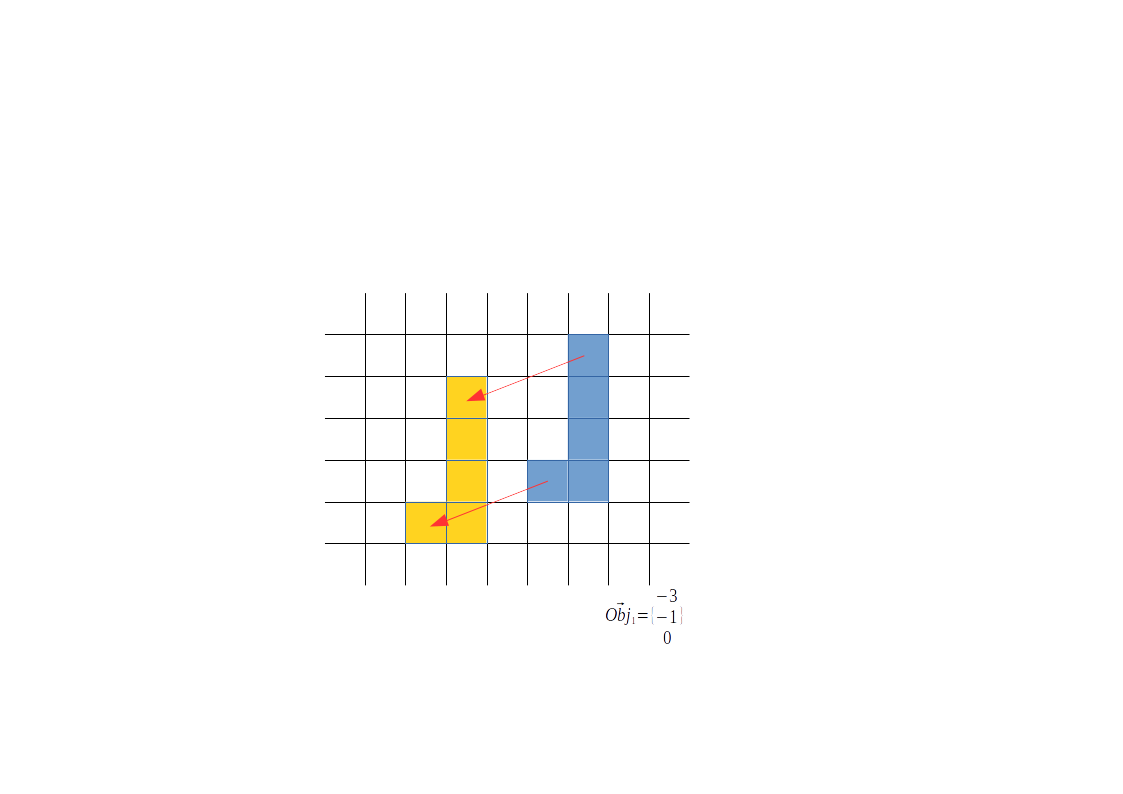
\includegraphics[width=0.9\linewidth]{../media/vec-obj1}
\caption[Vektor Objekt]{Vektordarstellung der Bewegung eines Objekts.}
\label{fig:vec-obj1}
\end{figure}

%\begin{itemize}
%\item Klassifizierung durch bewegungsmuster
%\item Voraussetzung Die Bewegung von Objekten nachvollziehen.
%\item Ansatz über Mittelpunkt beobachten
%\item woher weiß ich ob Mp in F1 = Mp in F2?
%\item Wie macht man Objekte einzigartig; ID?
%\item Verschiebung von Mittelpunkt vpn P1 in F1 zu P2 in F2 gibt Richtung und sogar Geschwindigkeit an.
%\item Darstellung als Vector; Orientierung und Länge = Richtung und Geschwindigkeit
%\item schema in visio
%\end{itemize}
\subsection{Konzept Hindernis umfahren}
Das Umfahren von Hindernissen ist nur bei statischen Objekten sinnvoll. Das Verhalten mobiler Objekte lässt sich nur schwer schätzen. Für die Modellierung von Ausweichrouten eignen sich Baiser Kurven. Die benötigten Start und Endpunkte der Kurve sind bereits bekannt. Hierfür können die aktuelle Position des Roboters und die Zielkoordinate des Roboters benutzt werden. Bezier Kurven werden über Hilfspunkte aufgespannt. Je mehr Hilfspunkte bekannt sind desto stärker wird die Kurve gekrümmt. Geeignete Hilfspunkte können auf einfache Art berechnet werden. Das Objekt liegt auf der Verbindungsachse zwischen mobiler Plattform und Zielpunkt. Nun kann vom Mittelpunkt des Störobjekts ein Vector aufgespannt werden der orthogonal auf die Verbindungsachse zeigt. Dieser Vector wird nun um den Durchmesser des Objekts Verlängert. Dadurch kann nun eine Kurve aufgespannt werden, die weit genug um das Hindernis herumführt, sodass der Roboter keine Gefahr läuft hängen zu bleiben.
\begin{figure}[H]
\centering
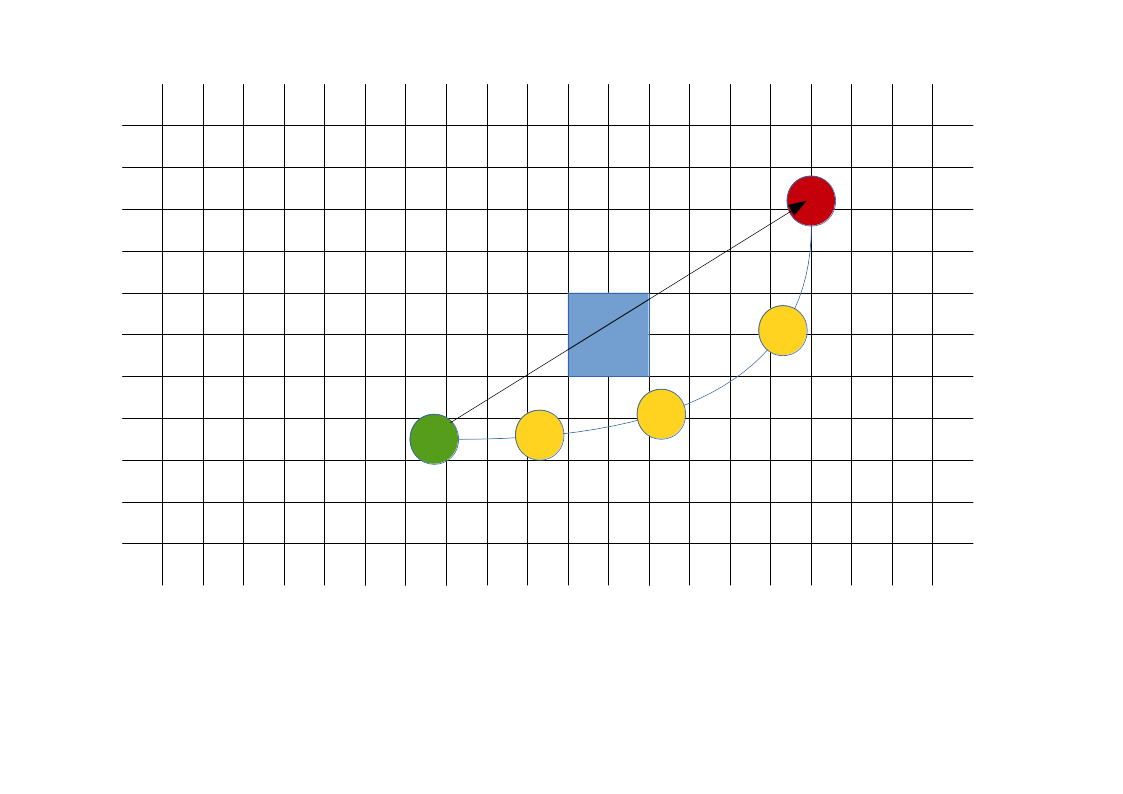
\includegraphics[width=0.9\linewidth]{../media/obj-curve}
\caption{Umfahrung eines Störobjekts, Streckenermittlung per Bezier-Kurve.}
\label{fig:obj-curve}
\end{figure}
